\documentclass[a4paper,twoside=false,abstract=false,numbers=noenddot,
titlepage=false,headings=small,parskip=half,version=last]{scrartcl}

\usepackage[utf8]{inputenc}
\usepackage[T1]{fontenc}
\usepackage[english]{babel}

\usepackage[colorlinks=true, pdfstartview=FitV,
linkcolor=black, citecolor=black, urlcolor=blue]{hyperref}
\usepackage{verbatim}
\usepackage{graphicx}
\usepackage{multirow}

\usepackage{tikz}
\usetikzlibrary{matrix}

\usepackage{amsmath}
\usepackage{amsthm}
\usepackage{amssymb}
\usepackage{amsfonts}


\theoremstyle{definition}
\newtheorem{exercise}{Exercise}

\theoremstyle{remark}
\newtheorem*{solution}{Solution}
\newtheorem*{remark}{Remark}

\newtheorem{theorem}{Theorem}[section]
\newtheorem{lemma}[theorem]{Lemma}
\newtheorem{proposition}[theorem]{Proposition}
\newtheorem{corollary}[theorem]{Corollary}

\newcommand{\NN}{\ensuremath{\mathbb{N}}}
\newcommand{\ZZ}{\ensuremath{\mathbb{Z}}}
\newcommand{\QQ}{\ensuremath{\mathbb{Q}}}
\newcommand{\RR}{\ensuremath{\mathbb{R}}}
\newcommand{\CC}{\ensuremath{\mathbb{C}}}
\newcommand{\GG}{\ensuremath{\mathcal{G}}}
\newcommand{\Fourier}{\ensuremath{\mathcal{F}}}
\newcommand{\Laplace}{\ensuremath{\mathcal{L}}}

\DeclareMathOperator{\Hom}{Hom}
\DeclareMathOperator{\End}{End}
\DeclareMathOperator{\im}{im}
\DeclareMathOperator{\id}{id}

\renewcommand{\labelenumi}{(\alph{enumi})}

\author{Jim Holmström - 890503-7571}
\title{Image Based Recognition and Classification - DD2427}
\subtitle{Exercise 6}

\begin{document}

\maketitle
\thispagestyle{empty}

\subsection{run}
    \verbatiminput{../src/run.m}

\subsection{LoadData}
    \verbatiminput{../src/LoadData.m}

\subsection{PerceptronLearning}
    \verbatiminput{../src/PerceptronLearning.m}

\subsection{TestHyperPlane}
    \verbatiminput{../src/TestHyperPlane.m}

\subsection{Result}
    \verbatiminput{resultdata.dat}

\pagebreak
\begin{figure}[t]
    \vspace{-270pt}
    \begin{center}
        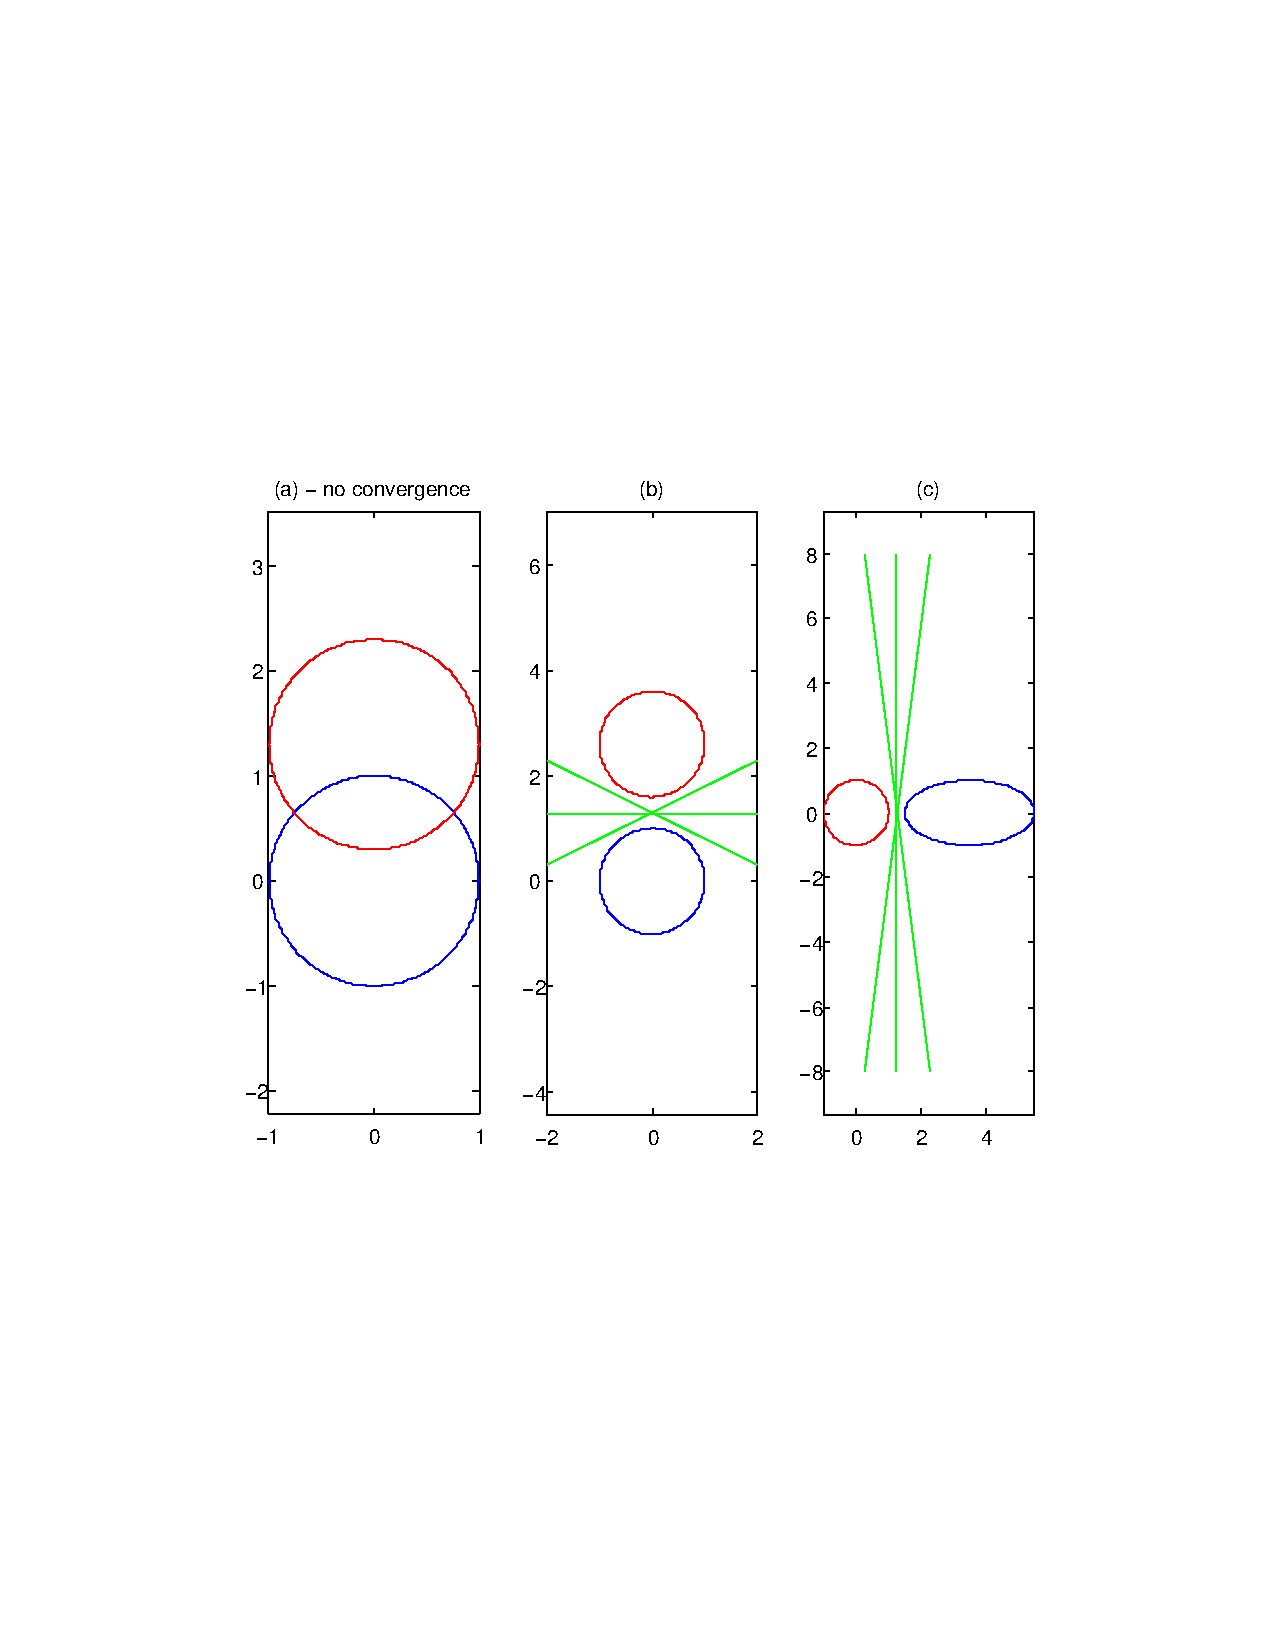
\includegraphics[width=1.0\textwidth]{linear_perceptron.pdf}
    \end{center}
    \vspace{-170pt}
    \caption{Linear Perceptron}
    \label{fig:linear}
\end{figure}
\begin{figure}[t]
    \vspace{-270pt}
    \begin{center}
        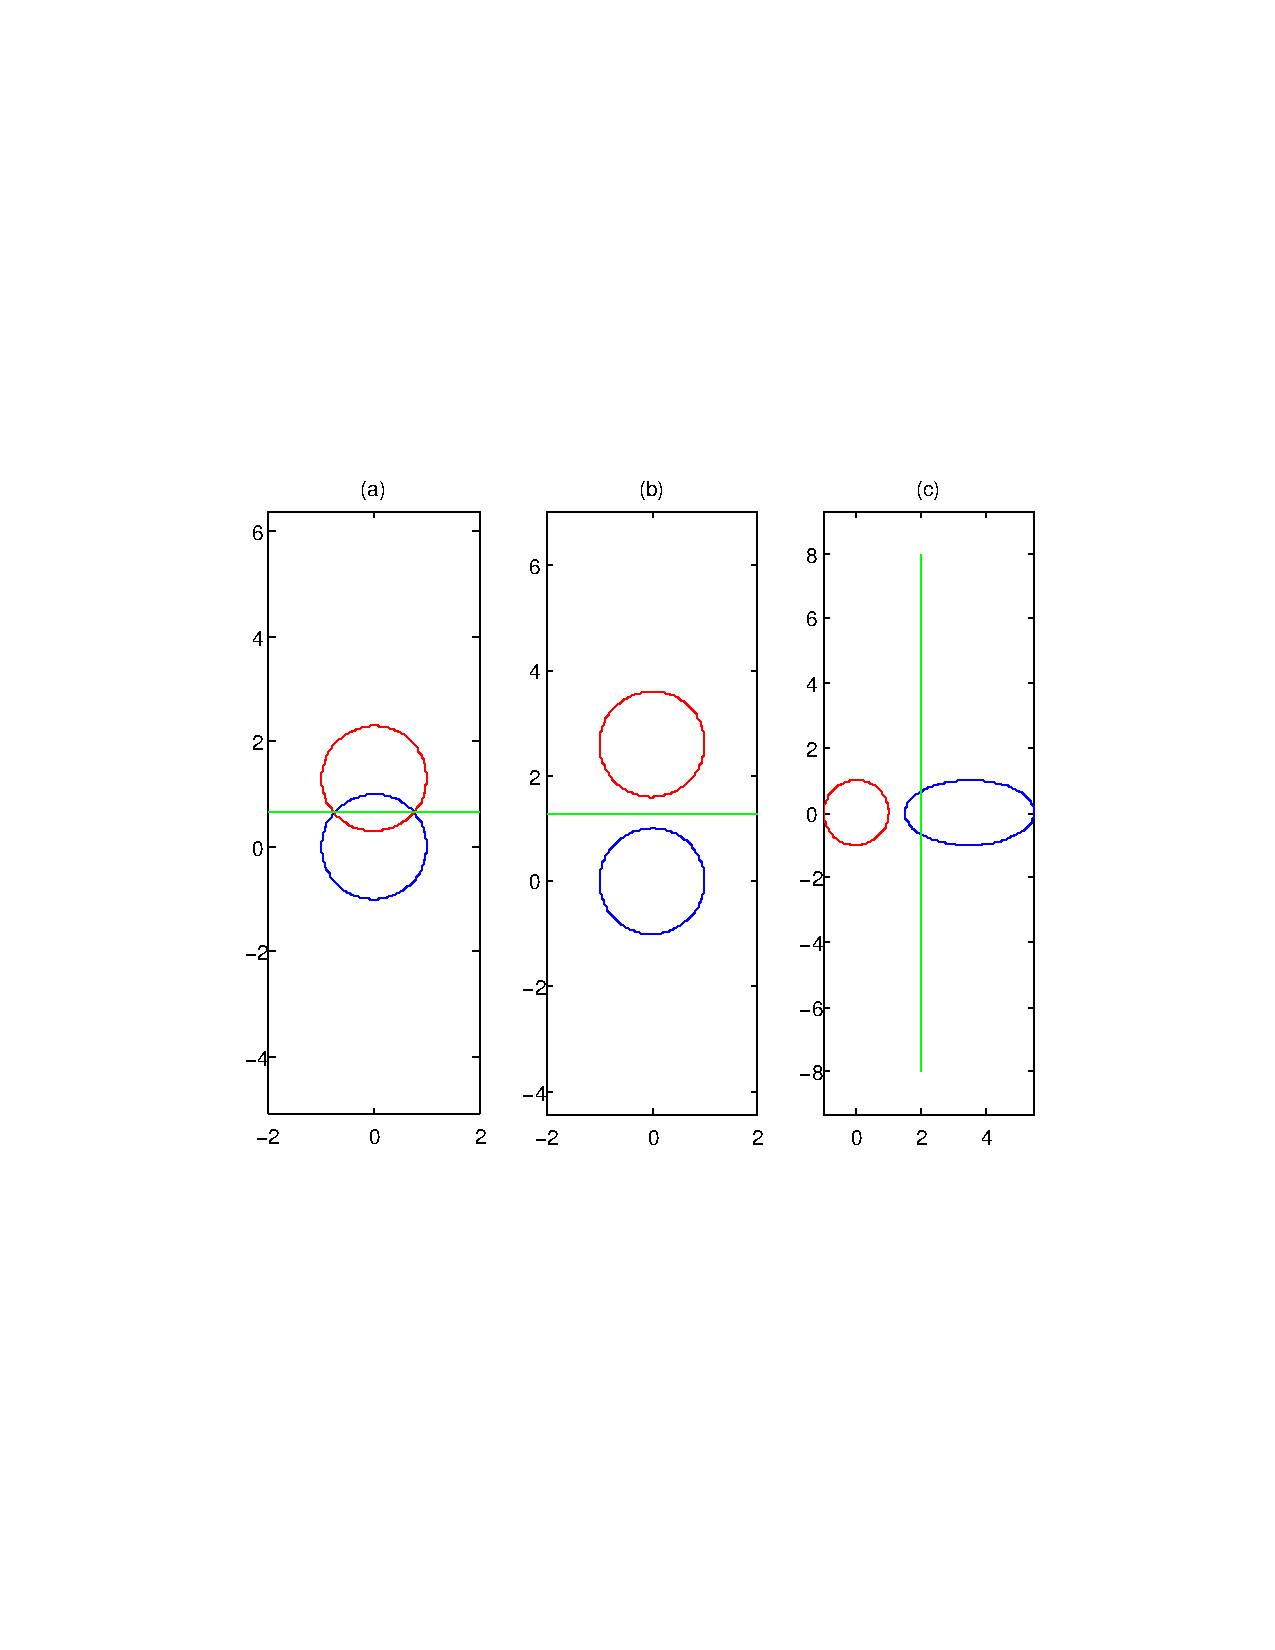
\includegraphics[width=1.0\textwidth]{minimum_square_error.pdf}
    \end{center}
    \vspace{-170pt}
    \caption{Minimum Square}
    \label{fig:square}
\end{figure}



\end{document}
